\section{Platforms, railings and stairs}

The standard platform used is a Bollegraaf design. The platforms are placed in Inventor, and no drawings are provided by Tebulo. Bolts are placed in the correct locations in the steel construction.

\begin{UNPPlatform}

Tebulo designed platforms are made out of UNP 160. To join the perpendicular UNP profiles, plates are welded in between the two, as shown in Figure \ref{fig:platformInternally}. When profiles are joined in the corner, the gap is bridged with a bigger plate as shown in Figure \ref{fig:platformCorner}.\\


\begin{minipage}[b]{.47\linewidth}
	\centering
	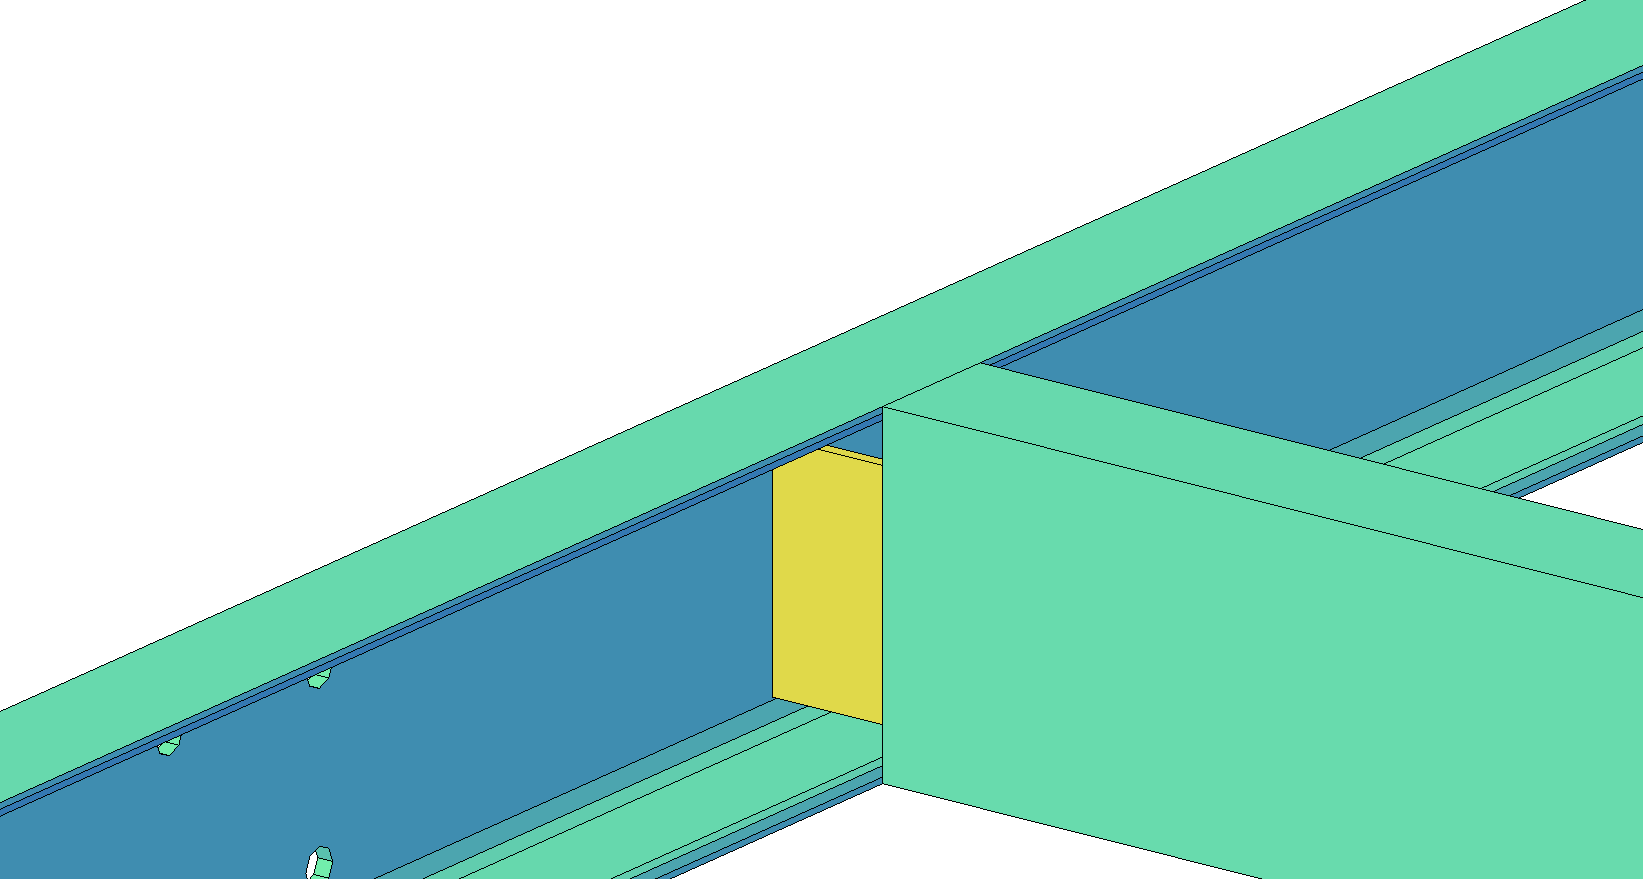
\includegraphics[width=\textwidth]{platformInternally}
	\captionof{figure}{The plates to connect internal perpendicular profiles in the platforms}\label{fig:platformInternally}
\end{minipage}
\qquad
\begin{minipage}[b]{.47\linewidth}
	\centering
	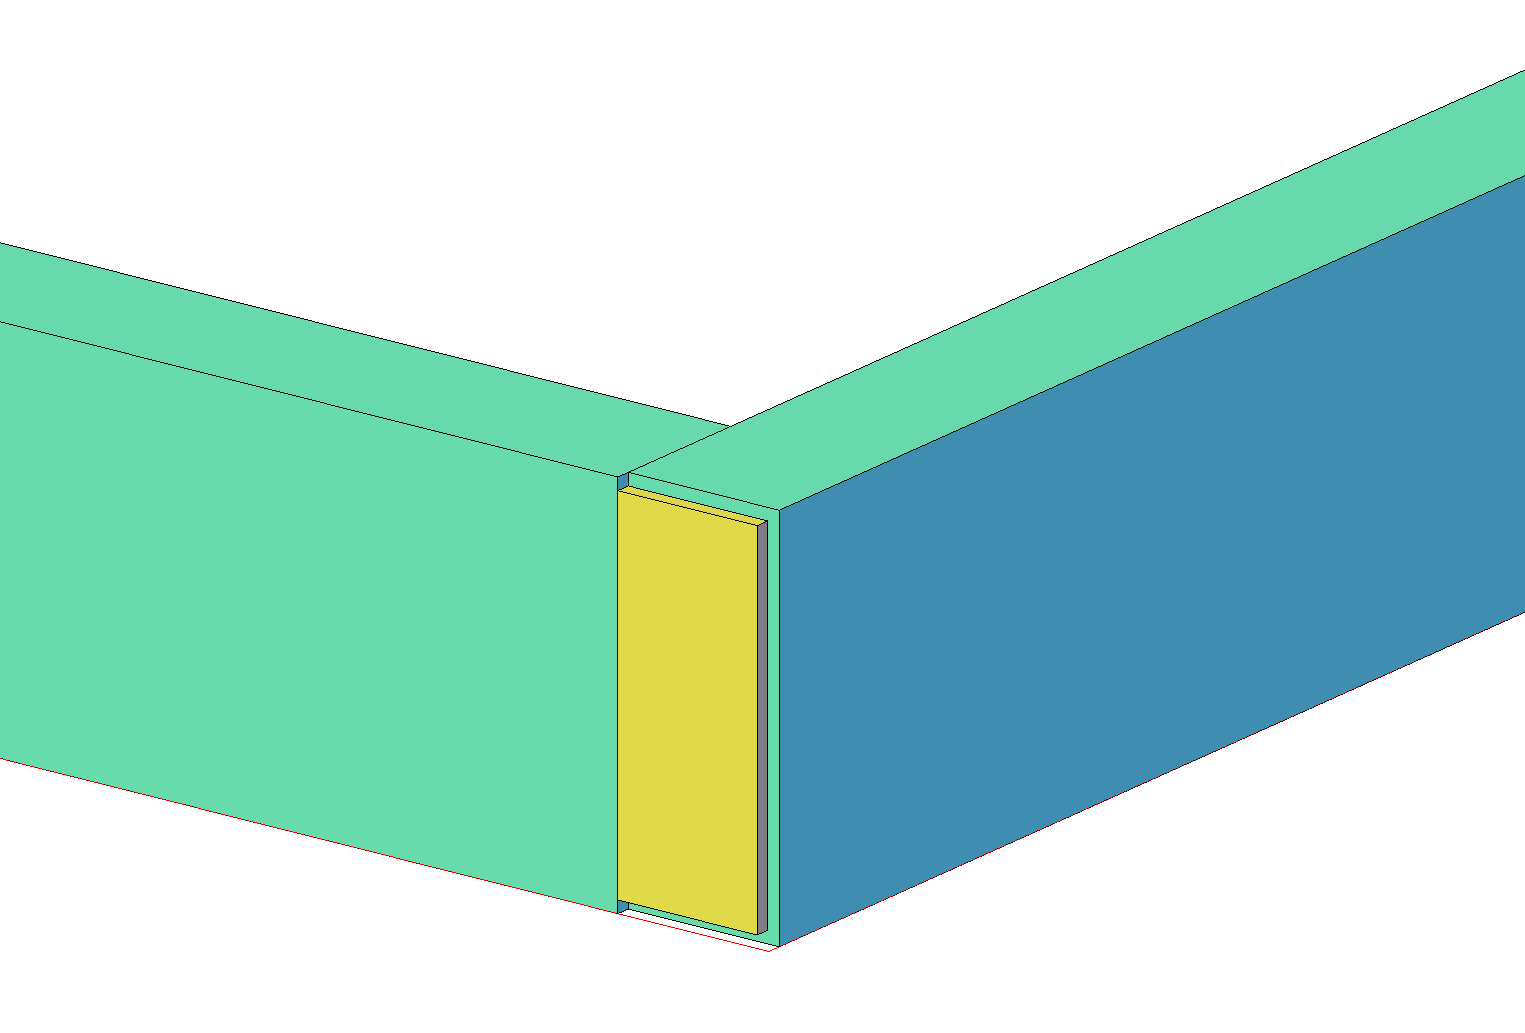
\includegraphics[width=\textwidth]{platformCorner}
	\captionof{figure}{The plates to connect UNP profiles in the platform corners}\label{fig:platformCorner}
\end{minipage}
%\vspace*{.5cm}


The platforms have hoisting eyes welded to the frame to lift them in place, as seen in Figure \ref{fig:platformHoisting}. The left plate is part of the handrail and kickplate. The full handrail can be seen in Figure \ref{fig:handrail}. The handrail is a design of Bollegraaf, and implemented by Tebulo.\\


\begin{minipage}[b]{.47\linewidth}
	\centering
	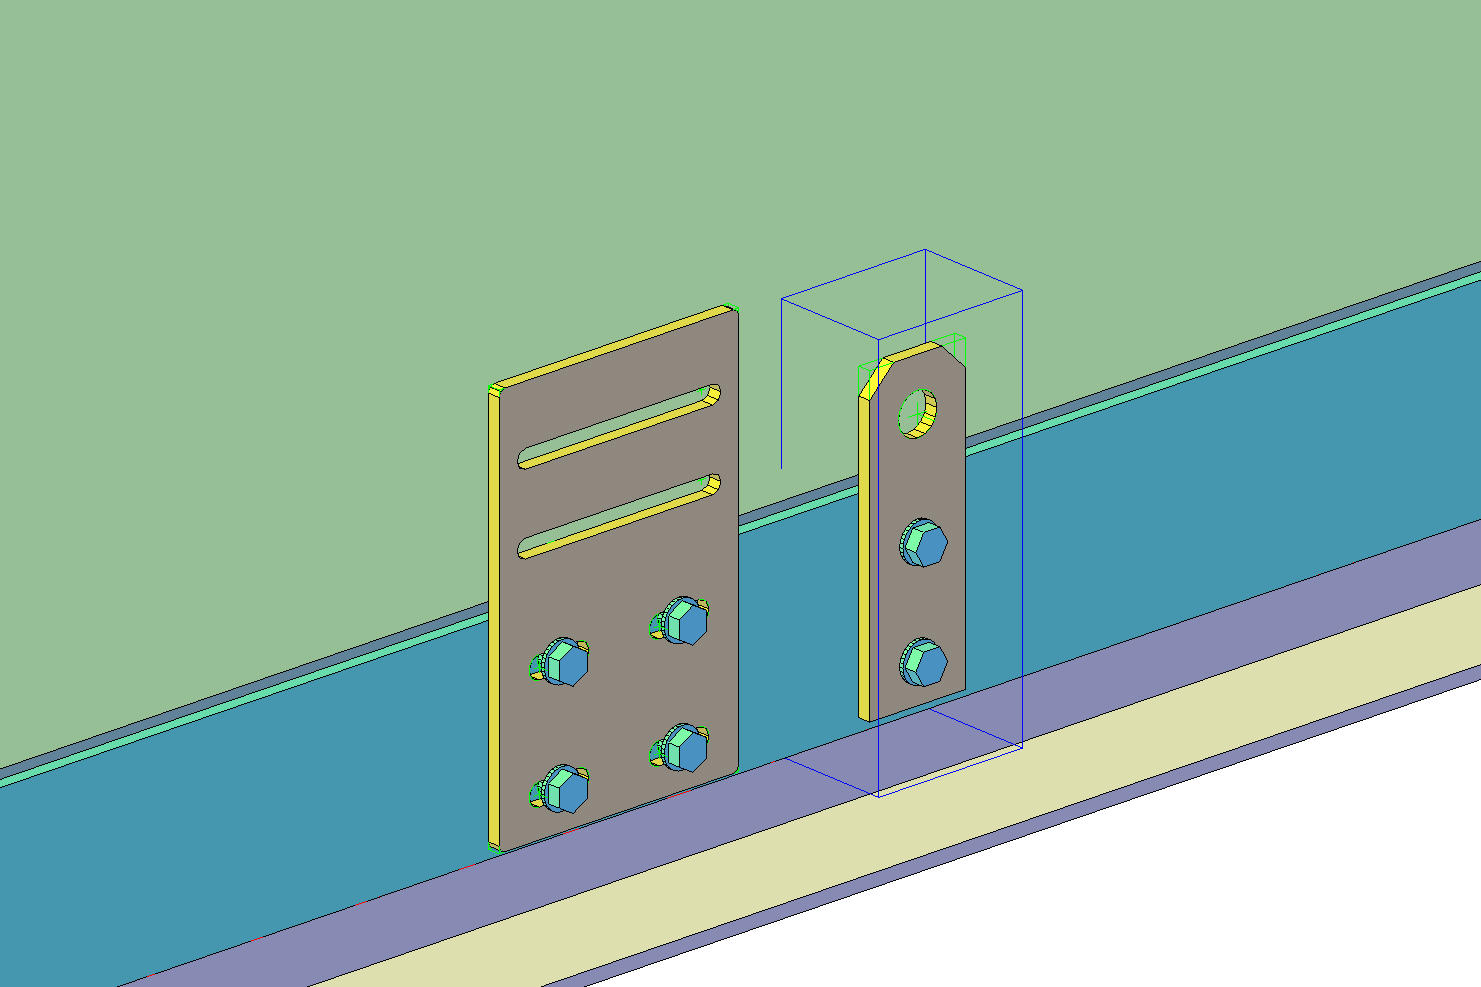
\includegraphics[width=\textwidth]{platformHoistingKickPlates}
	\captionof{figure}{A plate that serves as mounting point for the handrail and kickplate (left). The plates to hoist the platforms into place (Right)}\label{fig:platformHoisting}
\end{minipage}
\qquad
\begin{minipage}[b]{.47\linewidth}
	\centering
	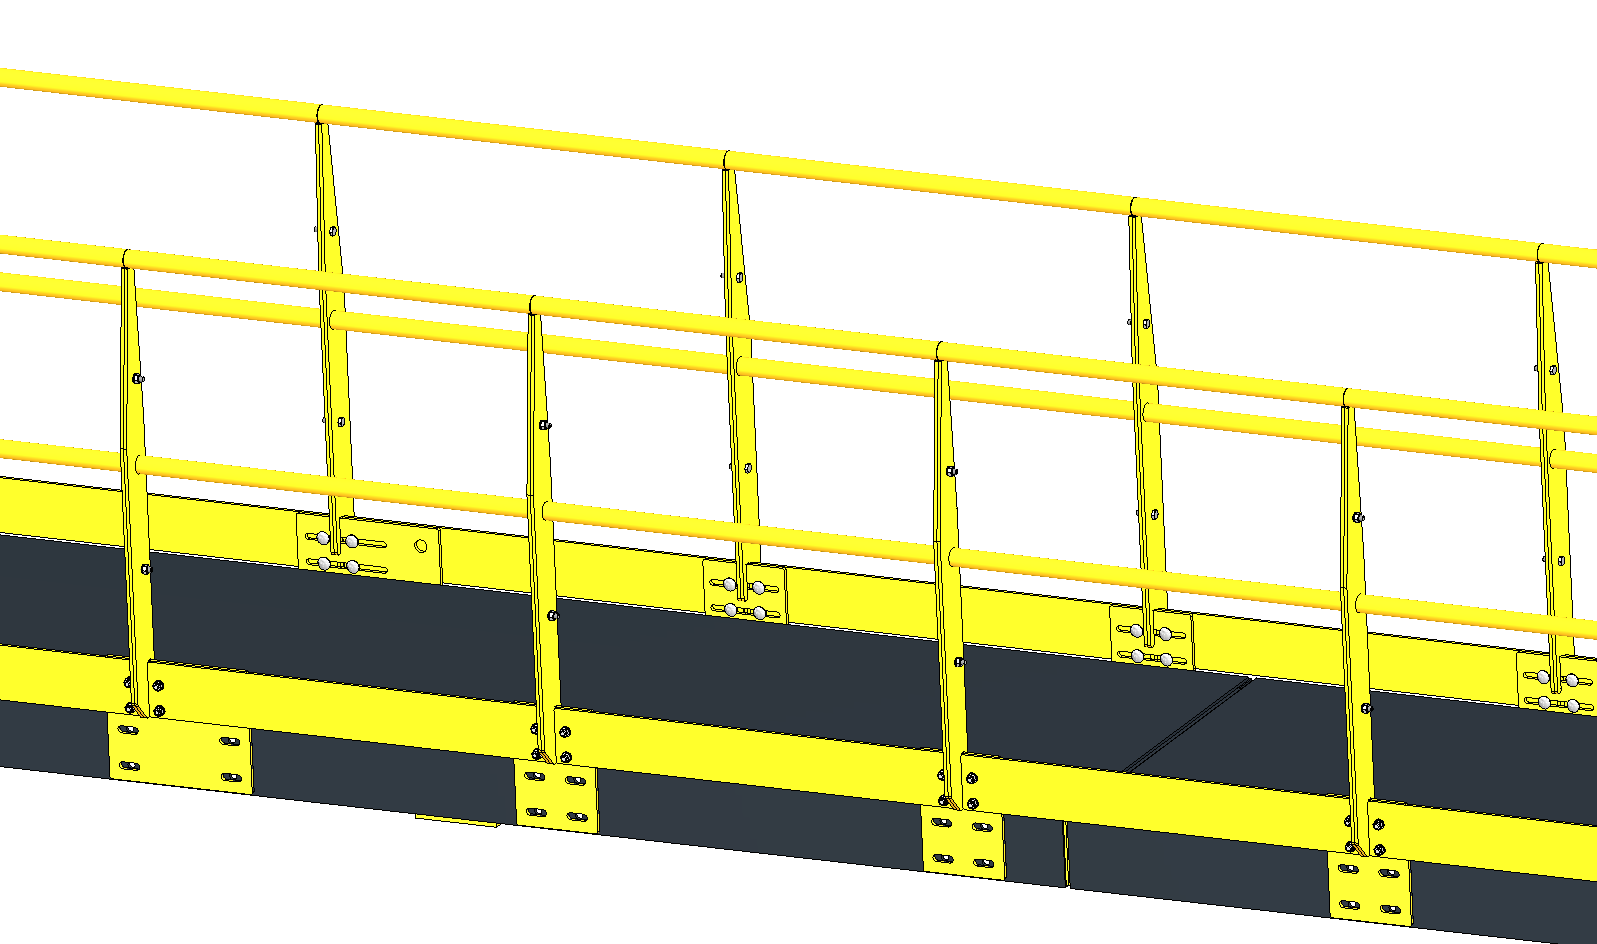
\includegraphics[width=\textwidth]{handrail}
	\captionof{figure}{The Bollegraaf handrail that is mounted on the UNP platforms}\label{fig:handrail}
\end{minipage}
\vspace{.5cm}


The grating placed on the platform has a thickness of 6mm, and is places 10mm from the edges. Furthermore space is reserved for machines and walkways wherever possible. \\
\end{UNPPlatform} \begin{visitorsPlatform}
If visitor platforms are present, they are constructed out of UNP 160 as well. This follows the same method of construction as the UNP platform, but has more requirements. These requirements follow either from \norm\ or agreements with Bollegraaf. These requirements in this project consist of a minimum width of 1.4m, and a different handrail with the bottom part closed off as seen in Figure \ref{fig:visitorPlatform}.

\begin{figure}[H]
\centering
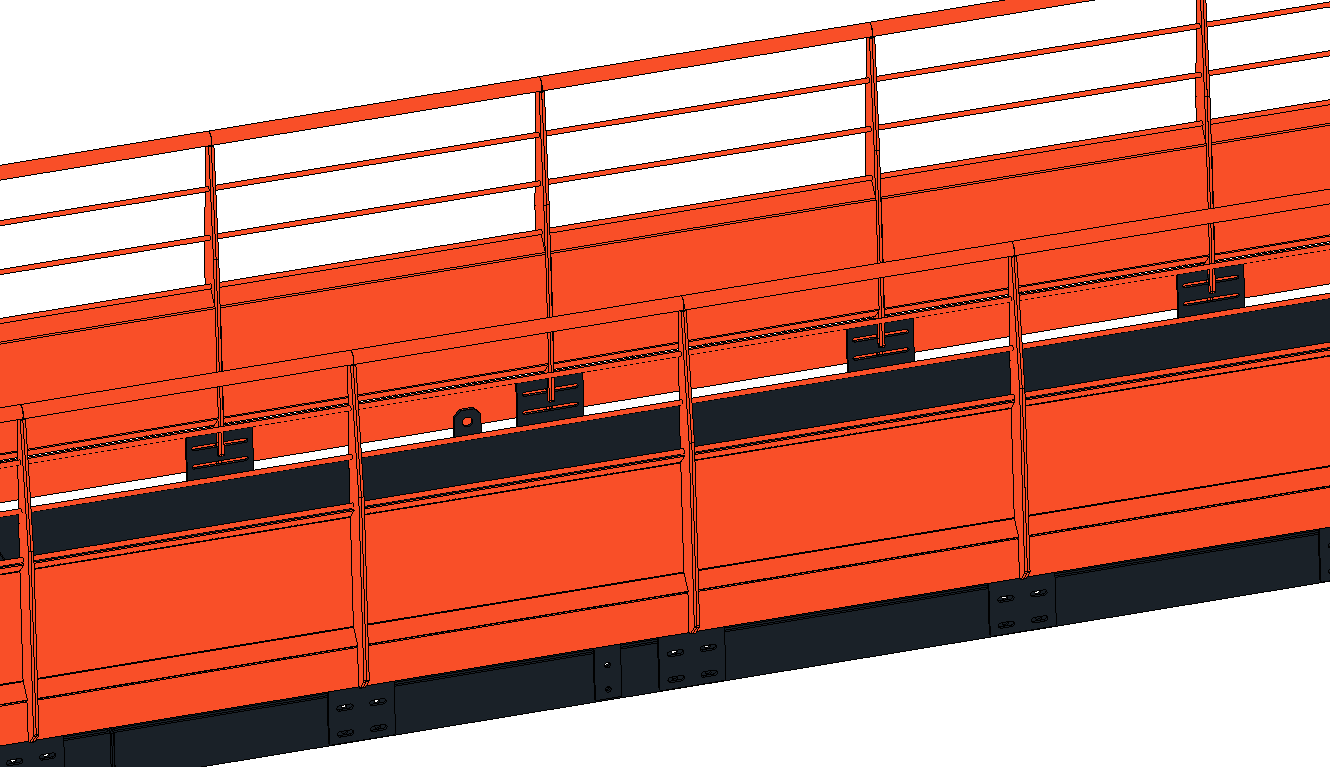
\includegraphics[width=.6\textwidth]{visitorPlatform}
\caption{The handrail used for visitor platforms}\label{fig:visitorPlatform}
\end{figure}

\end{visitorsPlatform}
